\documentclass[14]{article}
\usepackage{arxiv}
\usepackage[english, russian]{babel}
\usepackage[T1]{fontenc}
\usepackage{url}
\usepackage{booktabs}
\usepackage{amsfonts}
\usepackage{nicefrac}
\usepackage{microtype}
\usepackage{multicol}
\usepackage{wrapfig}
\usepackage{lipsum}
\usepackage{graphicx}
\usepackage{multicol}
\usepackage[justification=centering]{caption}
\usepackage{natbib}
\usepackage{doi}
\usepackage[utf8]{inputenc}
\usepackage{amsmath}
\usepackage{mathtools}
\usepackage{algpseudocode}
\usepackage{algorithm2e}
\usepackage{ dsfont }
\usepackage{setspace}


\title{Дистилляция знаний в глубоких сетях}

\author{ Михаил Олейник \\ 
  МФТИ \\
  \texttt{oleinik.ms@phystech.edu} \\
  \And
  М. Горпинич \\ 
  МФТИ \\
  \texttt{gorpinich.m@phystech.edu} \\
  \And
  О. Ю. Бахтеев \\ 
  МФТИ \\ 
  \texttt{bakhteev@phystech.edu} \\
}
\date{}

\renewcommand{\undertitle}{}
\renewcommand{\headeright}{}
\renewcommand{\shorttitle}{Дистилляция знаний в глубоких сетях}

\hypersetup{
pdftitle={Дистилляция знаний в глубоких сетях},
pdfauthor={Михаил Олейник},
pdfkeywords={дистилляция модели \and байесовский вывод \and глубокое обучение \and вариационная оптимизация},
}

\begin{document}
\maketitle

\begin{abstract}
  Дистилляция знаний позволяет повысить качество модели, называемой учеником, не увеличивая её число параметров,
  а используя модель большего размера, называемой учителем.
  Однако, в случае разных архитектур и несовпадения количества слоев у учителя и ученика, распространённые методы не применимы.
  Одним из подходов, который позволяет решать задачу для разных архитектур, является максимизация взаимной информации.
  Мы предлагаем улучшение этого подхода, которое позволит проводить дистилляцию и для моделей с разным количеством слоёв.
  Мы сравниваем наш метод с остальными с помощью вычиcлительного эксперимента.
  Также проводим анализ гиперпараметров и выводим ограничения на них, при которых достигается наибольшее качество.
\end{abstract}

\keywords{дистилляция модели \and байесовский вывод \and глубокое обучение \and вариационная оптимизация}


\section{Введение}
Глубокие нейронные достигли больших успехов в задачах машинного зрения, обработки естественного языка и других.
Однако, лучшие результаты достигают модели с большим количеством параметров,
из-за этого их трудно встроить в системы с небольшими вычислительными мощностями, например, мобильные телефоны.
Если подобрать размер модели под целевую платформу, уменьшив количество параметров, то сильно потеряем и в качестве.

Одним из подходов, которые позволяют не теряя сильно в качестве, получить модель с меньшим количеством параметров, является дистилляция знаний.
Этот подход использует большую предобученную на необходимой задаче модель, называемую учителем,
данные о слоях которой переносятся определенным образом в модель меньшего размера, называемую учеником.
Перенос чаще всего выражается в дополнительном слагаемом в функции потерь ученика.

Так, в работе \cite{hinton2015distilling} предлагается переносить знания с последнего слоя модели.
К недостаткам этого метода можно отнести то, что мы игнорируем информацию из остальных слоев учителя, а она может быть ценной.
В работах ...

Однако, большинство подходов либо неэффективно работают, либо не могут быть применимы к случаям, когда модели имеют разное количество слоёв или разную архитектуру.
Также возникают сложности в случае, когда количество параметров в слое учителя сильно больше,
чем в соответствующем слое ученика, как показано в работе \cite{mirzadeh2020improved}.

Больший интерес представляют подходы, которые можно применить, если учитель и ученик имеют разные архитектуры.
В работе \cite{passalis2020heterogeneous} моделируется информационный поток в учителе, который имитирует ученик.
В работе \cite{Ahn_2019_CVPR} используется максимизация взаимной информации между парами соответствующих слоёв.
В основе этого метода используется вариационный подход \cite{barber2004algorithm}.
Наша работа предлагает улучшение данного метода, давая возможность проведения дистилляции при разном количестве слоев у учителя и ученика.
Также мы проводим анализ гиперпараметров алгоритма, на примере работы \cite{gorpinich2022gradient}.

\section{Постановка задачи}

Дан датасет для задачи многоклассовой классификации, с количеством классов $K$:

$$\mathfrak{D}  = \{(\bold{x}_i, y_i)\}_{i=1}^{m},\; \bold{x}_i \in \mathbb{R}^n,\; y_i \in \mathbb{Y}  = \{1, \dots, K\},$$

Датасет разбит на обучающую и тестовую выборку: $\mathfrak{D} = \mathfrak{D}_\text{train} \bigsqcup \mathfrak{D}_\text{test}$.

Дана модель учителя $\bold{f}$, обученная на $\mathfrak{D}_\text{train}$.
Дана модель ученика $\bold{g}$, которую предстоит обучить.

Пусть $T$ --- количество слоев в модели учителя, $S$ --- количество слоев в модели ученика.
Обозначим как $t_i$ и $s_j$ --- активации в $i$-м слое учителя и в $j$-м слое ученика, соответственно.

Функцию потерь ученика представим как:

$$
  \mathcal{L} = \beta \mathcal{L}_\text{task} + (1 - \beta){\sum_{i, j=1}^{T, S}\lambda_{i, j}I(t_{i}, s_{j})},
$$
\noindent
где $\mathcal{L}_\text{task}$ --- функция потерь для решения задачи классификации,
$I(t_{i}, s_{j})$ --- взаимная информация, $\beta$ и $\lambda_{i, j}$ --- гиперпараметры.

\begin{figure}[h]
  \begin{multicols}{2}
    \hfill
    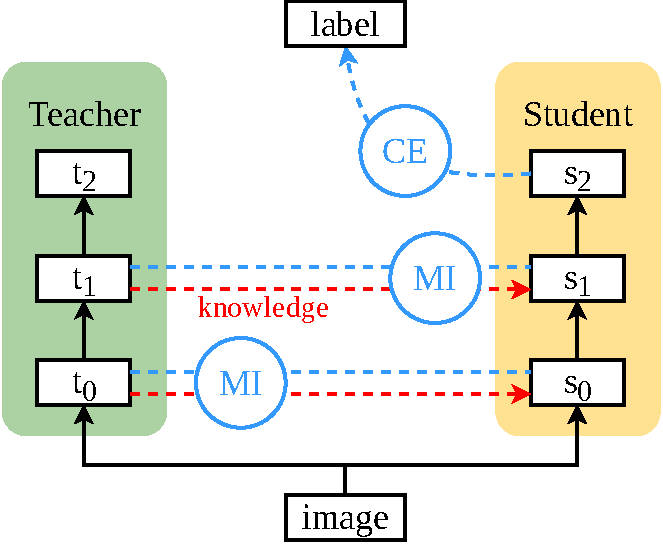
\includegraphics[width=0.4\textwidth]{../figures/ahn_diagram.pdf}
    \hfill
    \caption{Базовый метод.}
    \label{ris:ahn_diagram}
    \hfill
    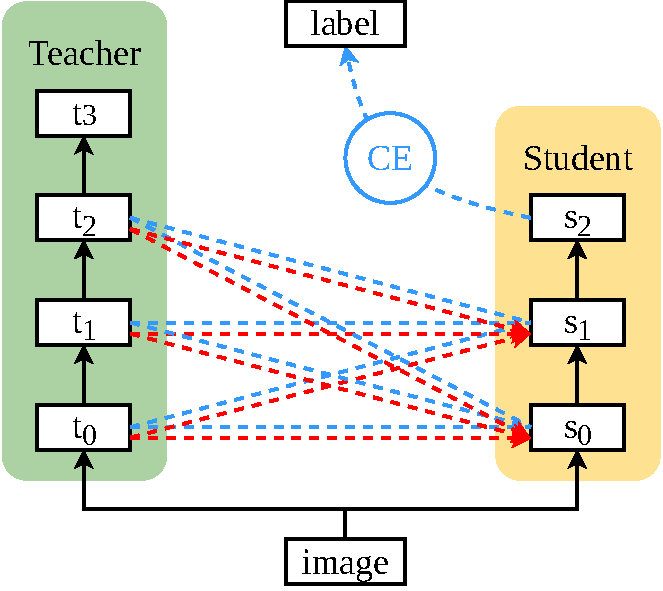
\includegraphics[width=0.4\textwidth]{../figures/our_diagram.pdf}
    \hfill
    \caption{Предлагаемый метод.}
    \label{ris:our_diagram}
  \end{multicols}
\end{figure}

\subsection{Взаимная информация}
Взаимная информация

\subsection{Алгоритм}
Алгоритм.
\section{Вычислительный эксперимент}

\begin{wrapfigure}{r}{0.25\textwidth}
  \begin{center}
    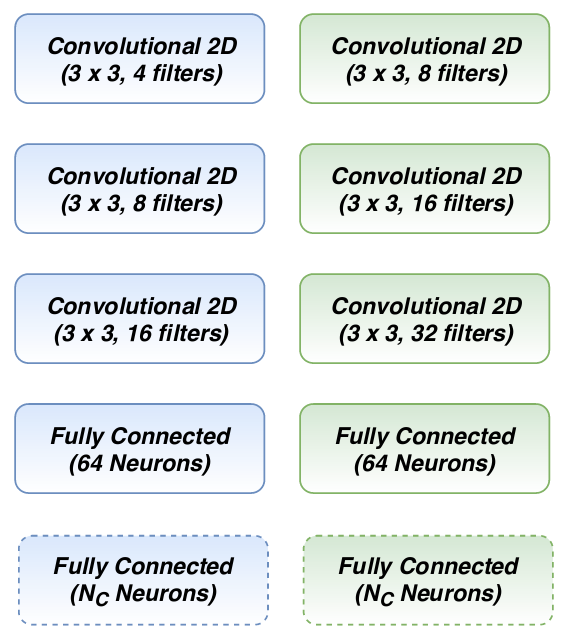
\includegraphics[width=0.25\textwidth]{../figures/conv_scheme.png}
  \end{center}
  \caption{Архитектура сетей \textbf{ConvTiny} и \textbf{ConvVeryTiny}.}
  \label{ris:conv_architecture}
\end{wrapfigure}

Для проведения экспериментов использовался датасет CIFAR10, разбитый на обучающую и тестовую выборку.
Использовались модели \textbf{ResNet10}, \textbf{ResNet18}, \textbf{ConvTiny} и \textbf{ConvVeryTiny}.
Последние две - свёрточные нейронные сети, с тремя свёрточными и двумя полносвязными слоями, как описано на схеме \ref{ris:conv_architecture}.


\subsection{Базовый эксперимент}

В качестве модели учителя была выбрана модель \textbf{ResNet18},
в качестве учеников --- \textbf{ConvTiny} и \textbf{ConvVeryTiny}.
В качестве метрики была выбрана точность (accuracy).

Цель --- сравнение качества учеников с и без дистилляции Хинтона, а также зависимость качества
дистиллированных моделей от гиперпараметров $\beta$ и $T$, что демонстрируется на графиках \ref{ris:hinton_box},
\ref{ris:hinton_beta} и \ref{ris:hinton_temp} соответственно.

\begin{figure}[h]
  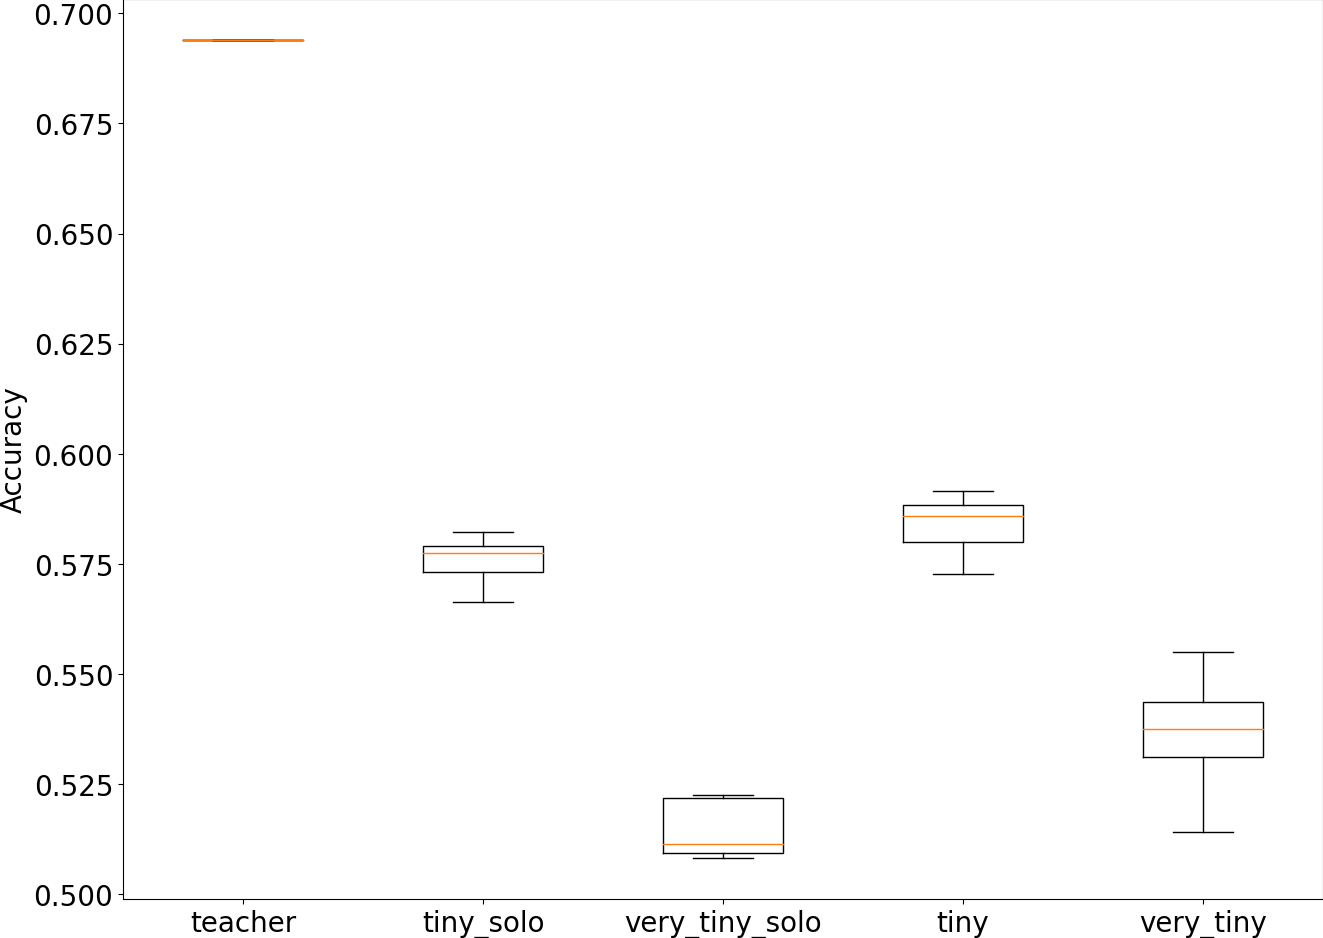
\includegraphics[width=9cm]{../figures/box_hinton_model_accuracy.png}
  \centering
  \caption{Сравнение качества моделей.}
  \label{ris:hinton_box}
\end{figure}

\begin{figure}[h]
  \begin{multicols}{2}
    \hfill
    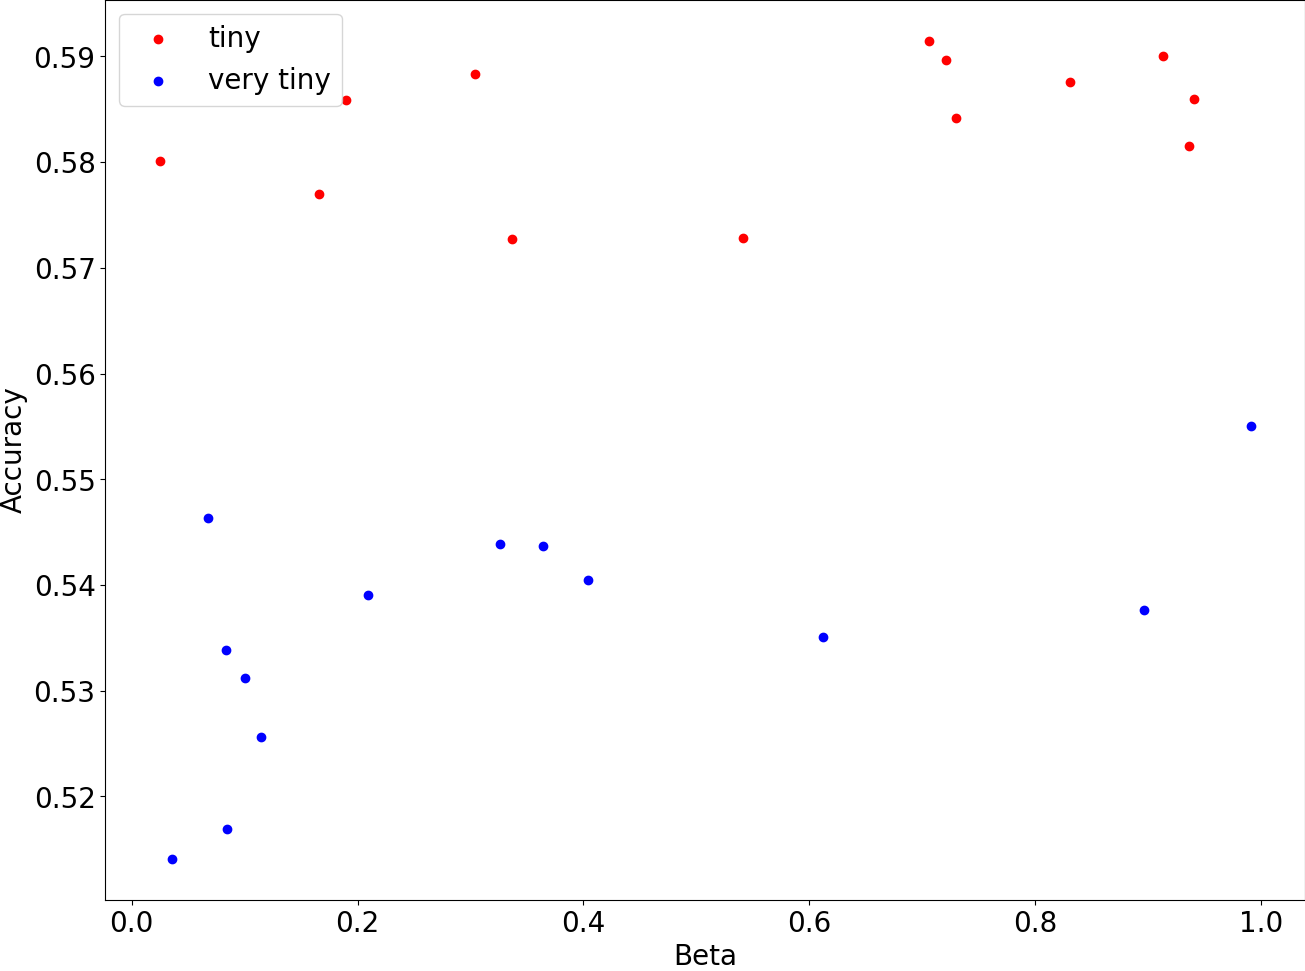
\includegraphics[width=0.5\textwidth]{../figures/scatter_hinton_beta_acc.png}
    \hfill
    \caption{Зависимость качества от параметра $\beta$.}
    \label{ris:hinton_beta}
    \hfill
    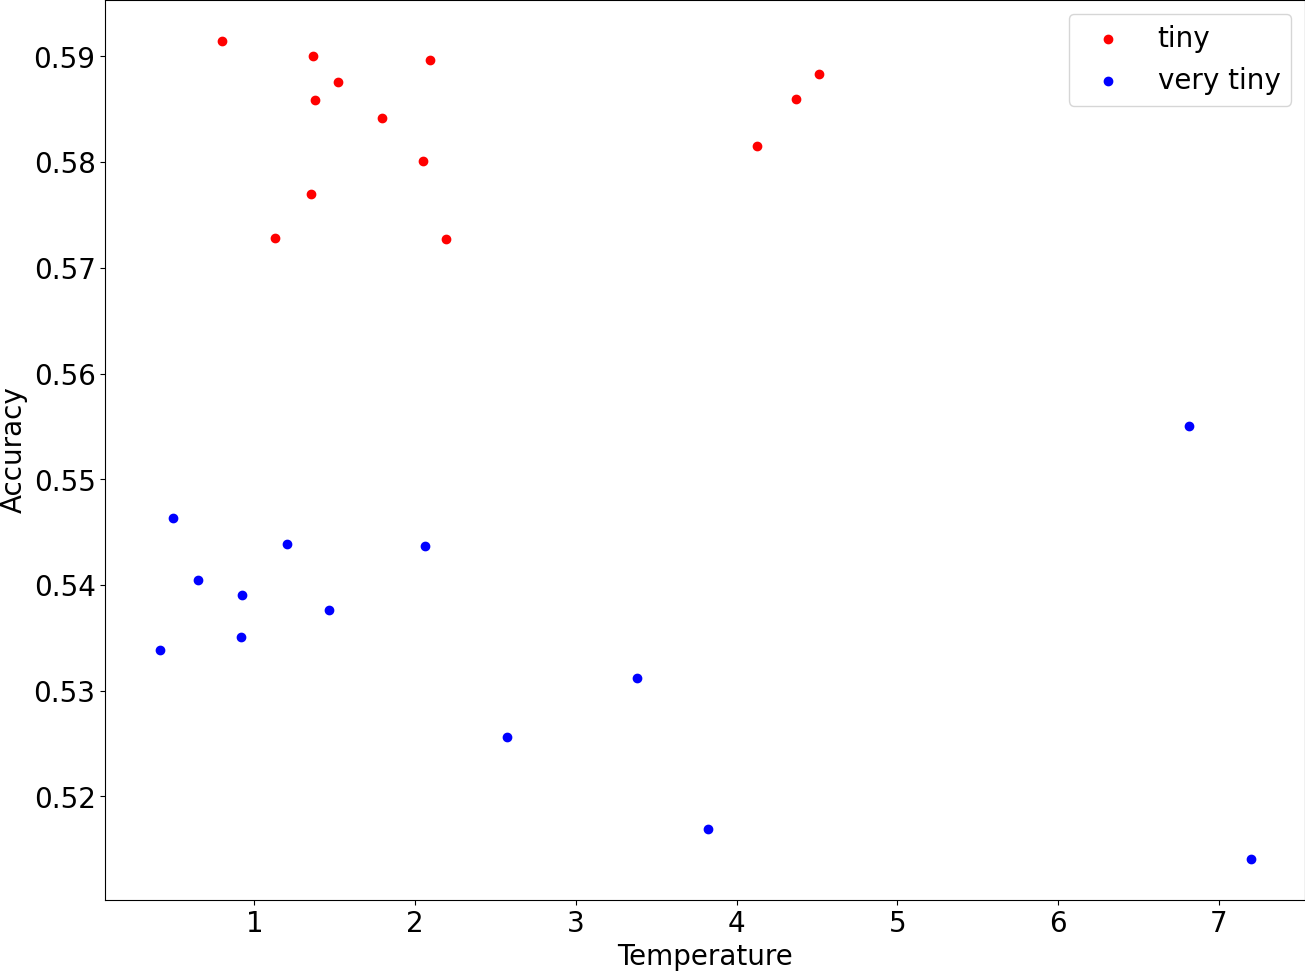
\includegraphics[width=0.5\textwidth]{../figures/scatter_hinton_temp_acc.png}
    \hfill
    \caption{Зависимость качества от параметра $T$.}
    \label{ris:hinton_temp}
  \end{multicols}
\end{figure}

\subsection{Основной эксперимент}

\subsubsection{Дистилляция из \textbf{ConvTiny}}

Был проведен эксперимент по дистилляции из \textbf{ConvTiny} в \textbf{ConvVeryTiny}.
Были рассмотрены разные методы: Хинтона, попарная, и предлагаемый метод.
В таблице \ref{table:tiny} представлены значения точности для моделей без дистилляции и при дистилляции упоминаемыми методами.


\begin{table}[h!]
  \centering
  \begin{tabular}{|l|l|l|l|l|}
    \hline
    Дистилляция & ---  & Хинтона & попарная  & каждый с каждым \\ \hline
    Учитель     & 0.58 & ---     & ---       & ---             \\ \hline
    Ученик      & 0.54 & 0.56    & 0.58-0.59 & 0.58-0.59       \\ \hline
  \end{tabular}
  \caption{Качество моделей при дистилляции на тестовой выборке, учитель --- \textbf{ConvTiny}, ученик --- \textbf{ConvVeryTiny}.}
  \label{table:tiny}
\end{table}

При предлагаемом методе дистилляции "каждый с каждым" выбирались случаные гиперпараметры $\lambda_{i, j}$
и $\beta$, на графике \ref{ris:tiny_accuracy} можно увидеть значение метрики на тестовой выборке для разных гиперпараметров,
на рисунке \ref{ris:tiny_lambdas} визуализированы значения $\lambda_{i, j}$ в лучших по качеству запусках.
Наблюдается общий паттерн, что связи с третьим слоем учителя (самым большим по количеству параметров)
больше, чем с остальными слоями учителя.

\begin{figure}
  \begin{minipage}[h]{0.35\linewidth}
    \center{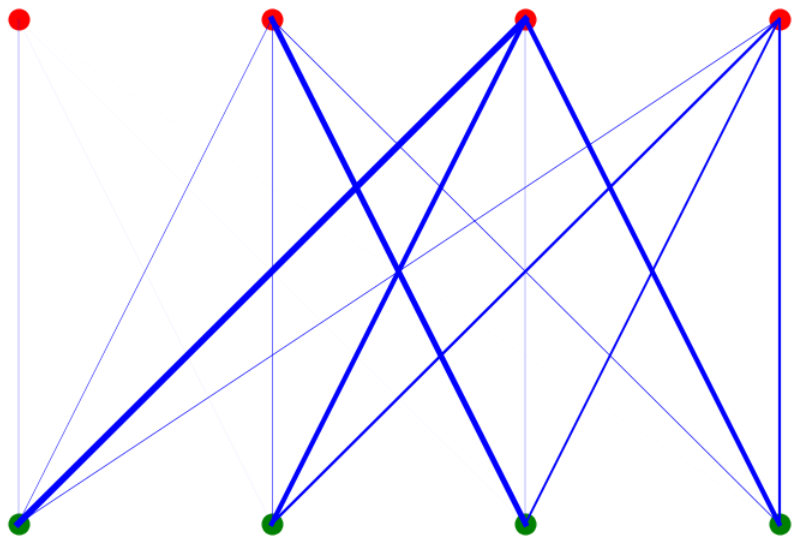
\includegraphics[width=1\linewidth]{../figures/connections_1}} a) \\
  \end{minipage}
  \hfill
  \begin{minipage}[h]{0.35\linewidth}
    \center{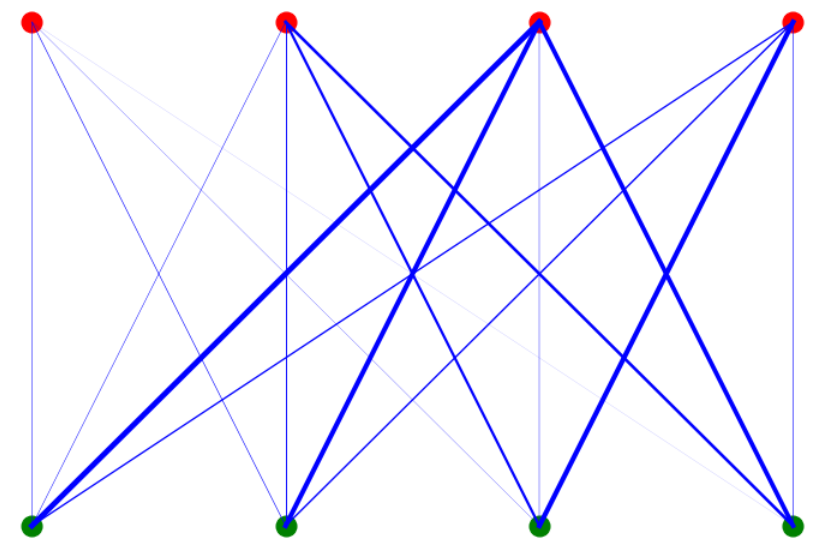
\includegraphics[width=1\linewidth]{../figures/connections_2}} b) \\
  \end{minipage}
  \vfill
  \begin{minipage}[h]{0.35\linewidth}
    \center{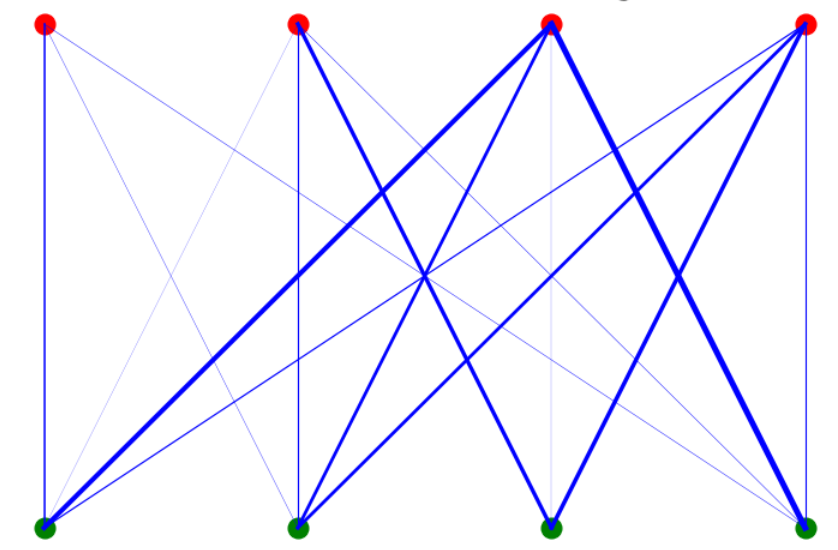
\includegraphics[width=1\linewidth]{../figures/connections_3}} c) \\
  \end{minipage}
  \hfill
  \begin{minipage}[h]{0.35\linewidth}
    \center{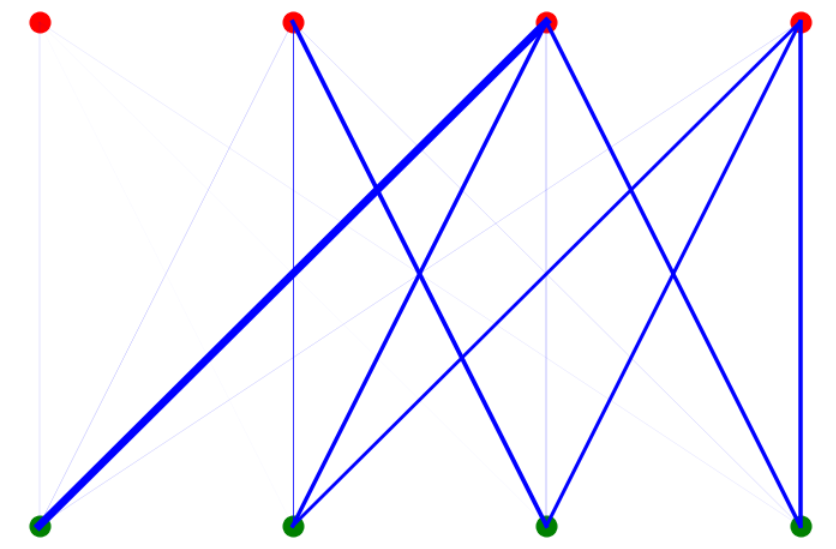
\includegraphics[width=1\linewidth]{../figures/connections_4}} d) \\
  \end{minipage}
  \caption{Иллюстрация коэффициентов у четырех лучших моделей по качеству. Зелёные точки --- слои ученика, красные --- слои учителя. Чем толще линия, тем больше коэффициент у соответствующей связи.}
  \label{ris:tiny_lambdas}
\end{figure}

\begin{figure}
  \center{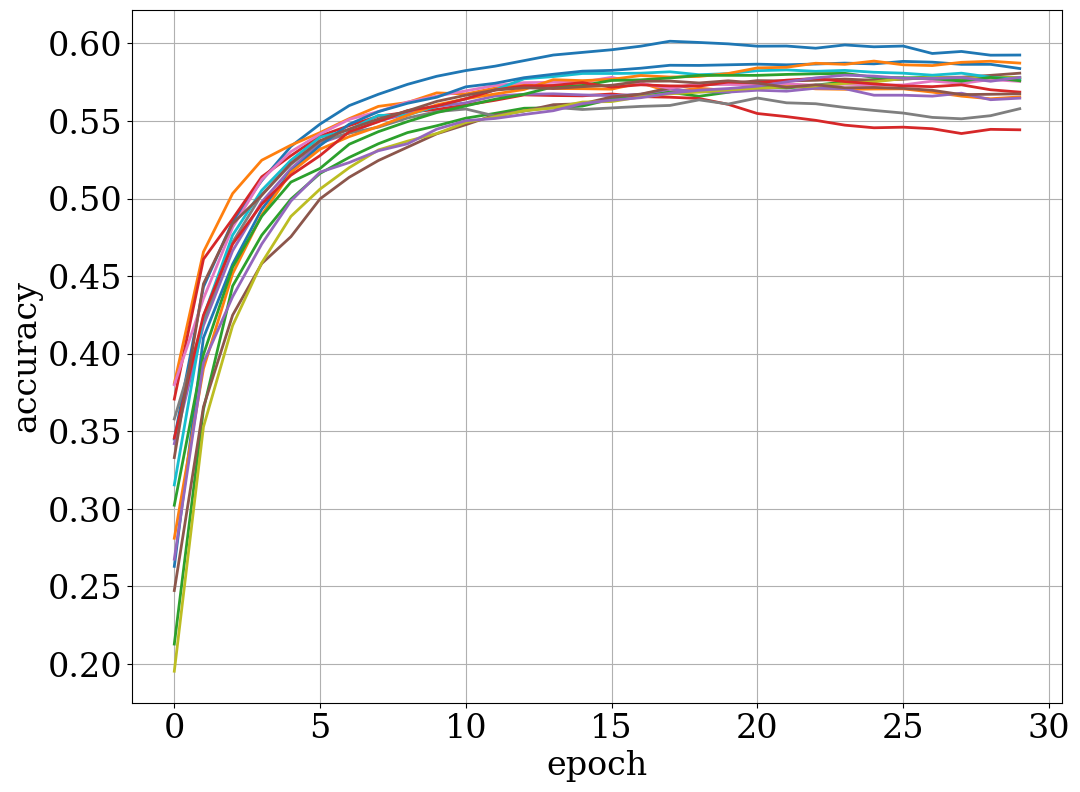
\includegraphics[width=0.7\textwidth]{../figures/distill_epoch_accuracy.png}}
  \caption{Точность от эпохи при дистилляции каждый с каждым}
  \label{ris:tiny_accuracy}
\end{figure}

\subsubsection{Дистилляция из \textbf{ResNet10}}

При дистилляции из \textbf{ResNet10} в \textbf{ConvVeryTiny} качество ухудшилось.
Это связано с тем, что сеть учителя стала слишком сложной для ученика,
данное явление рассматривается в работе \cite{mirzadeh2020improved}.

В таблице \ref{table:resnet10} представлены значения метрик при дистилляции из \textbf{ResNet10} в \textbf{ConvTiny}.


\begin{table}[h!]
  \centering
  \begin{tabular}{|l|l|l|l|}
    \hline
    Дистилляция & ---  & Хинтона & каждый с каждым \\ \hline
    Учитель     & 0.68 & ---     & ---             \\ \hline
    Ученик      & 0.58 & 0.60    & 0.63            \\ \hline
  \end{tabular}
  \caption{Качество моделей при дистилляции на тестовой выборке, учитель --- \textbf{ResNet10}, ученик --- \textbf{ConvTiny}.}
  \label{table:resnet10}
\end{table}

\section{Заключение}
Заключение.


\newpage
\bibliographystyle{unsrt}
\bibliography{references.bib}

\end{document}